\documentclass[conference]{IEEEtran}
\usepackage{amsmath,amssymb}
\usepackage{graphicx}
\usepackage{booktabs}
\usepackage{array}
\usepackage{url}
\usepackage{iftex}
\ifXeTeX
  \usepackage{fontspec}
  \setmainfont{texgyretermes}[Extension=.otf, UprightFont=*-regular, BoldFont=*-bold,
    ItalicFont=*-italic, BoldItalicFont=*-bolditalic]
\fi
\graphicspath{{figures/}}

\begin{document}

\title{Traffic Speed Forecasting on the METR-LA Road Network with Per-Sensor Tree Ensembles\\
\large Project 4: Traffic Flow Prediction and Signal Control via Graph Attention Networks and Flow Models --- Phase 1 (Machine Learning)}

\author{\IEEEauthorblockN{Team T072, Section C}
\IEEEauthorblockA{Rudraksh Sharma (2401010395), Anshuman Mehta (2401010082), Vridhi Chaudhary (2401010336),\\
Bineet Keshari (2401010130), Kavya Katal (2401020031)}}

\maketitle

\begin{abstract}
Traffic congestion builds up and spreads across a road network within minutes, so reliable short-term forecasts are the first step towards any traffic-control strategy. In Phase 1 of this project we build a complete, leakage-safe machine-learning pipeline that forecasts the speed at each of the 207 road sensors of the METR-LA dataset 5 to 60 minutes ahead. We compare two simple references (persistence and a training-only historical average) with two tree ensembles: a multi-output Random Forest per sensor and a direct XGBoost model per sensor and horizon. Both learned models use the same 38 causal features built from a 60-minute history window. Data are split strictly by time, with purged boundaries, and sensor outages are masked rather than treated as zero speed. On the test period, XGBoost gives the lowest mean absolute error (MAE) at every headline horizon: 2.92, 3.38 and 3.87 mph at 15, 30 and 60 minutes, which is 16.1\%, 19.1\% and 27.2\% lower than persistence. Random Forest gives the lowest root mean squared error (RMSE) and is more accurate than XGBoost during 60-minute peak-hour forecasts. Error maps show that the largest errors cluster along particular corridors. This supports the project hypothesis that independent per-sensor models miss congestion spreading between neighbouring roads, which Phase 2 will address with a graph attention network.
\end{abstract}

\begin{IEEEkeywords}
traffic forecasting, METR-LA, Random Forest, XGBoost, chronological validation, missing-data masking
\end{IEEEkeywords}

\section{Introduction}
Urban traffic is a network problem: when one road segment slows down, the queue grows backwards into upstream roads and the effect is felt elsewhere minutes later. Traffic agencies need short-term speed forecasts to warn drivers, plan diversions and, in the long run, adapt traffic signals.

Project 4 asks us to predict congestion on a road network and to test whether graph-based learning improves on independent road-segment forecasts. Any signal control must be simulated only. The faculty brief splits this into two parts:
\begin{enumerate}
\item an \emph{ML baseline} using lagged and time-of-day features with XGBoost per segment or a multi-output Random Forest (this report, Phase 1);
\item a \emph{deep-learning model}, a Graph Attention Network (GAT) or diffusion graph model, over the road graph (Phase 2).
\end{enumerate}

This report covers Phase 1 only. Our contributions are:
\begin{itemize}
\item a verified data pipeline for METR-LA (207 sensors, 34,272 five-minute time steps) with outage masking and a rebuilt road adjacency matrix that matches the published one;
\item 38 causal features, including cyclic time-of-day and time-of-week encodings, computed without using any future information;
\item four forecasting methods compared on exactly the same target points, with MAE, RMSE and MAPE reported for each horizon, for peak and off-peak hours, and per sensor;
\item congestion and error maps showing where independent models fail, which sets up the Phase 2 graph model;
\item a tested, reproducible code base with run manifests, 56 unit and integration tests, and continuous integration.
\end{itemize}

Table~\ref{tab:requirements} maps each requirement in the faculty instructions and project brief to the section of this report that addresses it.

\begin{table*}[t]
\centering
\caption{Where each Phase 1 requirement is addressed}
\label{tab:requirements}
\begin{tabular}{p{0.30\textwidth}p{0.42\textwidth}p{0.18\textwidth}}
\toprule
Requirement (source) & What we did & Section \\
\midrule
Literature review (rubric) & Eleven sources covering traffic forecasting, tree ensembles, metrics, graph models and simulation & \ref{sec:lit} \\
Dataset quality and EDA (rubric) & Shape, frequency, sensor order, missingness, outages, daily profiles, congestion map & \ref{sec:data} \\
Feature engineering (rubric); lagged and time-of-day features (brief) & 12 lags, missing flags, rolling statistics, cyclic time features; feature importance & \ref{sec:features} \\
Theoretical rigor (rubric) & Problem formulation, bagging and boosting theory, loss functions, metric definitions & \ref{sec:method} \\
Model application (rubric); XGBoost per segment or multi-output RF (brief) & Both models plus two references, validation-only tuning & \ref{sec:method}, \ref{sec:results} \\
Chronological splits, never random (brief) & Time-ordered 70/10/20 split with purged boundaries & \ref{sec:splits} \\
Fit scaling only on training data (brief) & No scaler needed; all fitted statistics (medians, historical averages) use training data only & \ref{sec:splits} \\
Mask sensor outages, do not treat as zero (brief) & 0 mph and NaN readings masked in inputs and targets & \ref{sec:data}, \ref{sec:features} \\
MAE, RMSE, MAPE by horizon; equal history windows (brief) & All 12 horizons, same 60-minute window for every model & \ref{sec:results} \\
Peak versus off-peak performance (brief) & Peak, off-peak, weekday and weekend slices & \ref{sec:results} \\
Congestion maps and horizon-wise metrics (brief deliverable) & Congestion map and per-sensor error maps on the road graph & \ref{sec:data}, \ref{sec:results} \\
Identify the gap of independent models (brief) & Spatial error clustering and discussion & \ref{sec:gap} \\
GitHub repository and code quality (rubric) & Modular package, tests, CI, pinned environment, provenance & \ref{sec:repro} \\
Individual contribution (instructions \S7) & Module ownership and pull requests & \ref{sec:team} \\
\bottomrule
\end{tabular}
\end{table*}

\section{Problem Statement}
Let $v_{t,i}$ be the measured speed (mph) at sensor $i\in\{1,\dots,207\}$ and time step $t$, sampled every 5 minutes. At a forecast origin $t$ we use the last 12 readings of the same sensor (the past 60 minutes) and the calendar time of $t$, and predict the next 12 readings:
\begin{equation}
\hat v_{t+h,i}=f_{i,h}\big(\phi(v_{t-11:t,\,i},\;c_t)\big),\qquad h=1,\dots,12,
\end{equation}
where $\phi$ is the feature map (Section~\ref{sec:features}) and $c_t$ is the calendar time. We report horizons $h=3,6,12$, i.e.\ 15, 30 and 60 minutes ahead, as headline results and keep all 12 horizons in the figures. This is a regression problem; the outputs are speeds, not classes, so ``accuracy percentages'' do not apply.

In Phase 1 each sensor is modelled \emph{independently}: no model sees the speed of neighbouring sensors. This is exactly the baseline the brief asks for, and it lets Phase 2 measure how much a graph model adds.

\section{Literature Review}
\label{sec:lit}
\textbf{Classical traffic forecasting.} Williams and Hoel \cite{williams} modelled freeway traffic as a seasonal ARIMA process and showed that strong daily and weekly cycles make recent history plus time of day very informative. Castro-Neto et al. \cite{castro} showed that forecasting quality differs between typical and atypical conditions (such as incidents and holidays), which motivates our separate peak, off-peak, weekday and weekend evaluation.

\textbf{Tree ensembles.} Random Forests \cite{breiman} average many decorrelated regression trees trained on bootstrap samples, which lowers variance and copes well with nonlinear relations and noisy inputs. XGBoost \cite{chen} builds trees one after another, each correcting the errors of the previous ones, with a regularised objective and efficient handling of sparse data. Both work directly on tabular lag features and need no feature scaling.

\textbf{Forecast evaluation.} Hyndman and Koehler \cite{hyndman} showed that percentage errors such as MAPE become unstable when true values are near zero and that different error measures can rank methods differently. We therefore report MAE, RMSE and MAPE together and mask zero-speed readings.

\textbf{Graph models for traffic.} DCRNN \cite{li} introduced METR-LA as a benchmark and modelled traffic as a diffusion process on a directed road graph built with a Gaussian distance kernel; we rebuild that same adjacency matrix. Graph Attention Networks \cite{gat} learn attention weights over each node's neighbours, so the model can decide how much each upstream or downstream sensor matters. This is the Phase 2 model suggested by the brief.

\textbf{Traffic flow theory and simulation.} The Lighthill--Whitham--Richards (LWR) model \cite{lighthill,richards} describes traffic as a conserved flow in which congestion travels as waves along a road. This is the physical reason why neighbouring sensors carry predictive information. CityFlow \cite{cityflow} and SUMO \cite{sumo} are traffic simulators for testing signal-control policies safely, without touching real traffic; they are relevant to the optional simulated signal experiment in Phase 2.

\textbf{Gap addressed.} Published graph models are usually compared with weak baselines, and differences in splits and masking make results hard to compare. We first build strong, well-validated non-graph baselines on a leakage-safe protocol, so that any later graph improvement can be measured fairly.

\section{Dataset and Exploratory Data Analysis}
\label{sec:data}
\subsection{Dataset}
METR-LA \cite{li} contains loop-detector speed readings from 207 sensors on Los Angeles County highways. The brief recommends it as the starter dataset because it comes with a road graph. Table~\ref{tab:data} summarises the file we used; all values were checked by our loader and audit scripts.

\begin{table}[t]
\centering
\caption{METR-LA dataset summary (verified by our loader)}
\label{tab:data}
\resizebox{\columnwidth}{!}{%
\begin{tabular}{ll}
\toprule
Property & Value \\
\midrule
Sensors (nodes) & 207 \\
Time steps & 34,272 (every 5 min) \\
Period & 1 Mar 2012 00:00 -- 27 Jun 2012 23:55 \\
Measured channel & Speed only (mph) \\
Observed speed range & 0.33 -- 70 mph (non-zero readings) \\
Missing readings (0 mph or NaN) & 8.11\% overall, 7.13\% in training \\
Separate outage runs & 17,867 \\
Longest single outage & 5,800 min ($\approx$4 days) \\
Training steps with all sensors missing & 1,301 \\
Road graph edges (excl.\ self-loops) & 1,515 directed edges \\
\bottomrule
\end{tabular}}
\end{table}

\textbf{Speed only.} The brief lists flow and occupancy features, but METR-LA contains only speed. We do not invent flow or occupancy values. Speed, flow (vehicles per hour) and occupancy (fraction of time a detector is covered) are different physical quantities. PeMS, which the brief suggests as a later extension, would be needed for real flow and occupancy channels.

\subsection{Data quality checks}
Our loader (\texttt{src/trafficml/data/load.py}) reads the original HDF5 file directly and rejects the data if any of the following fail: the sensor order matches the graph's sensor list; timestamps are unique and exactly 5 minutes apart; there are no infinite or negative speeds. The road adjacency matrix rebuilt from the raw distance file with the Gaussian kernel $W_{ij}=\exp(-d_{ij}^2/\sigma^2)$ (weights below 0.1 set to zero) matches the published DCRNN matrix. The pickle loader only allows NumPy objects, so a malicious file cannot run code.

\textbf{Outages.} A reading of 0 mph means the sensor reported nothing, not that traffic stopped. We convert 0 and NaN to ``missing'' and never use them as real speeds or as targets. Fig.~\ref{fig:missing} shows that missing data come in two kinds: whole-network outages (vertical bands, e.g.\ around training days 25 and 38) and long outages of single sensors (horizontal streaks).

\begin{figure*}[t]
\centering
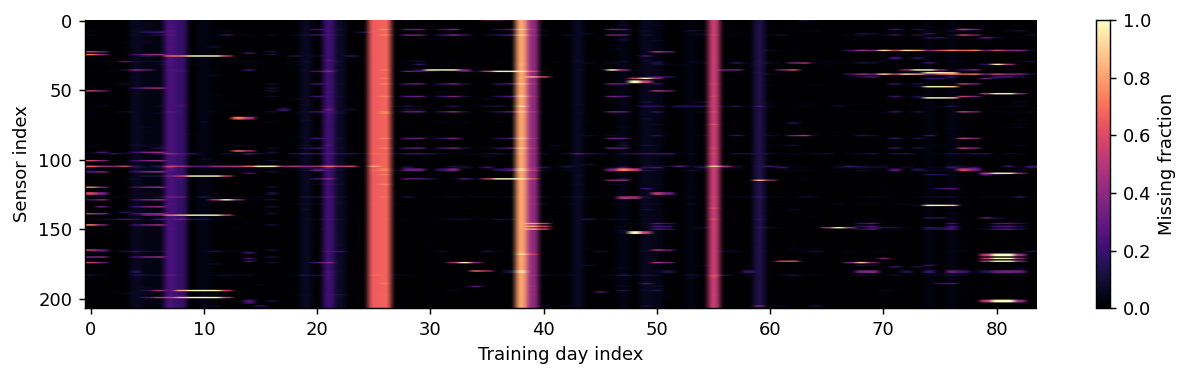
\includegraphics[width=0.85\textwidth]{missingness.png}
\caption{Fraction of missing readings per sensor and training day. Vertical bands are network-wide outages; horizontal streaks are single sensors failing for days.}
\label{fig:missing}
\end{figure*}

\subsection{Exploratory analysis}
All EDA uses the training period only, so the test period does not influence our design decisions.

\textbf{Daily pattern.} Fig.~\ref{fig:daily} shows clear weekday rush hours: the network-average speed falls from about 62 mph to about 49 mph in the morning (around 08:00--09:00) and to about 46 mph in the evening (around 17:30). Weekends have no morning dip and only a mild midday slowdown. This is why time-of-day and weekend features are useful, and why we evaluate peak and off-peak hours separately.

\begin{figure}[t]
\centering
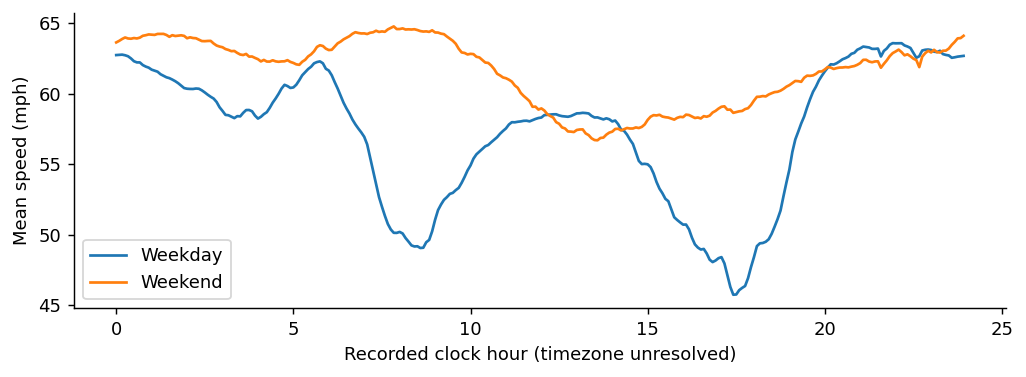
\includegraphics[width=\columnwidth]{daily_profile.png}
\caption{Mean training speed by recorded clock hour for weekdays and weekends.}
\label{fig:daily}
\end{figure}

\textbf{Network view.} Fig.~\ref{fig:heatmap} shows one training day for all sensors. Congestion appears as dark bands at the same times on many sensors, but with different start and end times. This suggests that congestion spreads between related sensors rather than appearing everywhere at once.

\begin{figure*}[t]
\centering
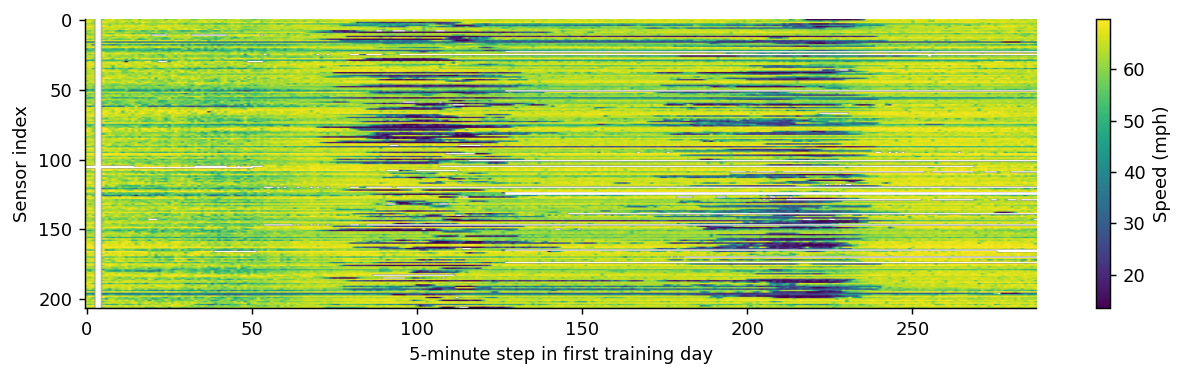
\includegraphics[width=0.85\textwidth]{speed_heatmap.png}
\caption{Speed of all 207 sensors over the first training day (288 five-minute steps). Dark bands are morning and evening congestion; white lines are missing readings.}
\label{fig:heatmap}
\end{figure*}

\textbf{Congestion map.} Fig.~\ref{fig:congestion} places every sensor on the map and draws the road-graph edges. Average speeds are lowest in the south-east (downtown) part of the network, where several highways meet, and highest on the eastern north--south branch.

\begin{figure}[t]
\centering
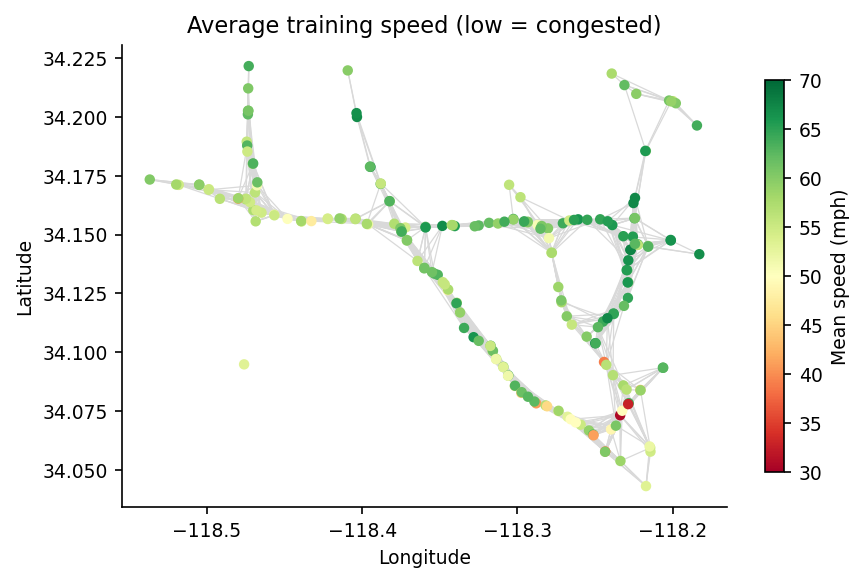
\includegraphics[width=\columnwidth]{congestion_map.png}
\caption{Congestion map: average training speed per sensor (red = slow). Grey lines are edges of the road graph built from road distances.}
\label{fig:congestion}
\end{figure}

\section{Feature Engineering}
\label{sec:features}
Each training example is one sensor at one forecast origin $t$. From the 12 most recent readings and the calendar time of $t$ we compute 38 features (Table~\ref{tab:features}). Every feature uses only information available at time $t$.

\begin{table}[t]
\centering
\caption{The 38 causal features}
\label{tab:features}
\footnotesize
\begin{tabular}{>{\raggedright\arraybackslash}p{0.4\columnwidth}c>{\raggedright\arraybackslash}p{0.36\columnwidth}}
\toprule
Group & Count & Purpose \\
\midrule
Speed lags $v_{t},\dots,v_{t-11}$ & 12 & Recent trend \\
Missing flags per lag & 12 & Tells the model a value was filled \\
Means of last 3, 6, 12 readings & 3 & Smoothed current level \\
Std, min, max of history & 3 & Volatility and range \\
Change over last step and whole window & 2 & Speeding up or slowing down \\
Missing fraction & 1 & Data reliability \\
$\sin,\cos$ of time of day & 2 & Daily cycle \\
$\sin,\cos$ of time of week & 2 & Weekly cycle \\
Weekend flag & 1 & Weekend behaviour \\
\midrule
Total & 38 & \\
\bottomrule
\end{tabular}
\end{table}

\textbf{Cyclic time.} Clock time is encoded as
\begin{equation}
x_{\sin}=\sin\!\left(\tfrac{2\pi\tau}{P}\right),\qquad x_{\cos}=\cos\!\left(\tfrac{2\pi\tau}{P}\right),
\end{equation}
where $\tau$ is the time within the period $P$ (one day or one week). This way 23:55 and 00:00 are close together, which they would not be with a plain hour number.

\textbf{Missing inputs.} Inside each 12-step window a missing reading is filled with the most recent earlier reading (forward fill only, never backward). If the window starts with missing readings, the sensor's training-period median is used. The missing flags record which values were filled. Targets are never filled: a missing target is simply not scored.

\textbf{Road-segment information.} Because a separate model is trained for each sensor, sensor-specific behaviour (typical speed, rush-hour pattern) is learned by that model. Neighbouring sensors' speeds are deliberately excluded in Phase 1.

\textbf{Scaling.} Tree models split on thresholds, so feature scaling does not change them and no scaler is used. All fitted statistics, i.e.\ the medians above and the historical-average tables, are computed from the training period only.

Fig.~\ref{fig:importance} shows which features the trained models rely on. Both depend mostly on the latest speed and the short rolling means. Random Forest also uses time-of-day features strongly; XGBoost uses the weekend flag and the longer history mean.

\begin{figure*}[t]
\centering
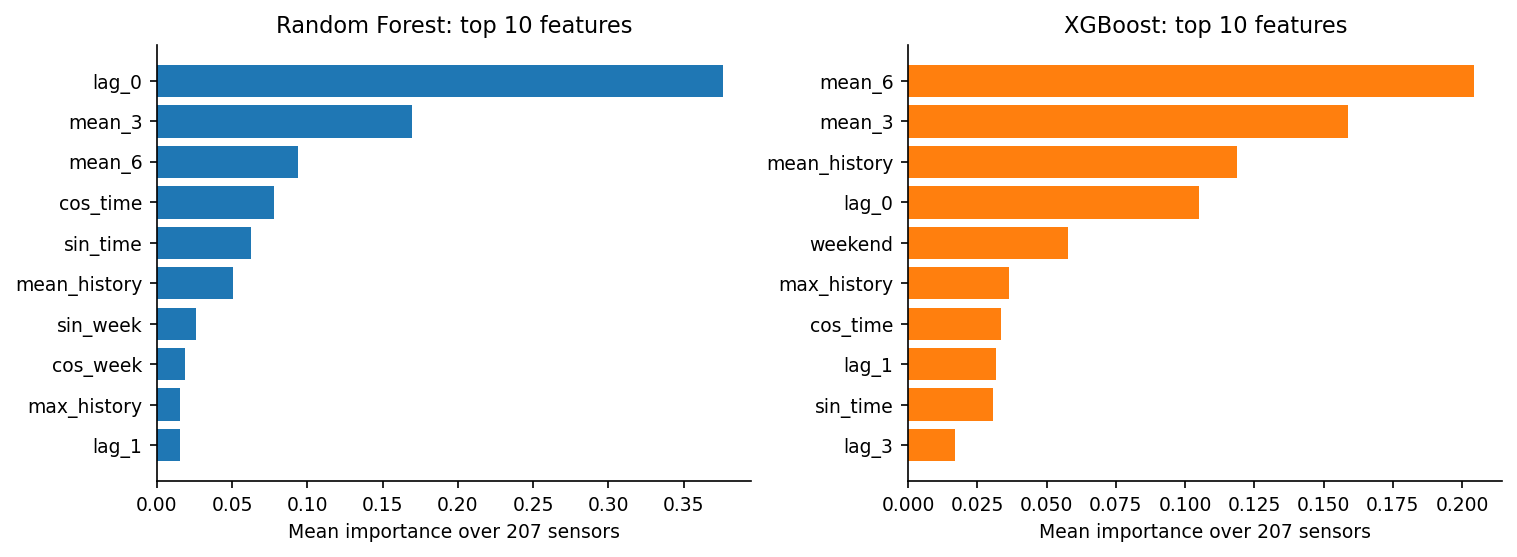
\includegraphics[width=0.8\textwidth]{feature_importance.png}
\caption{Top 10 features, averaged over the 207 sensor models (impurity reduction for Random Forest, gain for XGBoost). Importance shows what a model uses, not cause and effect.}
\label{fig:importance}
\end{figure*}

\section{Methodology}
\label{sec:method}
\subsection{Chronological splits and leakage prevention}
\label{sec:splits}
Random splitting would leak the future into training, because neighbouring time steps are almost identical. We therefore split forecast origins strictly in time: 70\% training, 10\% validation and 20\% test (Table~\ref{tab:splits}). The validation block is cut into two halves: \emph{val-tune} for choosing hyper-parameters and \emph{val-2} as a second, separately reported check.

A forecast made at the last training origin looks 12 steps ahead. Without care, those future targets would overlap the next block. We therefore remove (``purge'') the last 11 origins of each earlier block, so every training target ends no later than the first validation origin.

\begin{table}[t]
\centering
\caption{Chronological partitions (forecast origins)}
\label{tab:splits}
\begin{tabular}{lll r}
\toprule
Block & First origin & Last origin & Samples \\
\midrule
Train & 01 Mar 00:55 & 23 May 05:45 & 23,963 \\
Val-tune & 23 May 06:45 & 29 May 04:25 & 1,701 \\
Val-2 & 29 May 05:25 & 04 Jun 03:10 & 1,702 \\
Test & 04 Jun 04:10 & 27 Jun 22:55 & 6,850 \\
\bottomrule
\end{tabular}
\end{table}

Leakage safeguards, each covered by an automated test:
\begin{itemize}
\item features use only readings at or before the origin;
\item medians and historical averages are fitted on training data only;
\item hyper-parameters are selected on val-tune only, then frozen;
\item every model is scored on the same target array and the same mask of valid points.
\end{itemize}

\subsection{Reference methods}
\textbf{Persistence (M0)} predicts that the speed stays at the latest valid reading for all 12 horizons. It is hard to beat at very short horizons.

\textbf{Historical average (M1)} predicts the training-period average speed of that sensor for the same 5-minute slot of the week, falling back to the time-of-day and then the overall sensor average when a slot has no data. It captures the regular weekly pattern but ignores today's conditions.

\subsection{Random Forest (M3)}
For each sensor we train one Random Forest that outputs all 12 horizons at once (multi-output). Each tree is grown on a bootstrap sample of the training rows, and each split considers a random subset of features. Averaging $B$ trees $T_b$,
\begin{equation}
\hat{\mathbf y}=\frac1B\sum_{b=1}^{B}T_b(\mathbf x),
\end{equation}
reduces variance because the trees' errors are only partly correlated \cite{breiman}. Trees split to minimise squared error, so a forest predicts the conditional mean. Because one model predicts the whole 12-step vector, training rows with any missing future label are dropped (on average 89.65\% of rows remain usable).

\subsection{XGBoost (M4)}
For each sensor and each horizon we train a separate XGBoost model (direct multi-horizon strategy, $207\times12=2{,}484$ models). Boosting adds trees one at a time, each fitted to the remaining errors of the current ensemble \cite{chen}, minimising
\begin{equation}
\mathcal L=\sum_{j}\ell(y_j,\hat y_j)+\sum_{k}\Big(\gamma T_k+\tfrac12\lambda\lVert w_k\rVert^2\Big),
\end{equation}
where $T_k$ is the number of leaves of tree $k$, $w_k$ its leaf weights, and $\gamma,\lambda$ penalise complex trees. Each horizon only drops rows whose label at that horizon is missing (92.87\% of rows usable on average).

\subsection{Hyper-parameter selection}
We compared two predefined settings per model on six evenly spaced pilot sensors in val-tune, using MAE at 15, 30 and 60 minutes (Table~\ref{tab:tuning}). The better setting was then trained on all 207 sensors. This is a small, budgeted search, not an exhaustive one. Training uses every second origin to keep the run time manageable (about 15 minutes to fit all models and save their predictions); evaluation uses every origin.

\begin{table}[t]
\centering
\caption{Hyper-parameter candidates (validation MAE on pilot sensors)}
\label{tab:tuning}
\begin{tabular}{p{0.66\columnwidth}r}
\toprule
Candidate & Val.\ MAE \\
\midrule
RF: 48 trees, depth 12, min leaf 8, 80\% features (\textbf{chosen}) & 3.829 \\
RF: 64 trees, depth 16, min leaf 5, 80\% features & 3.881 \\
XGB: 100 trees, depth 3, lr 0.08, squared error & 3.824 \\
XGB: 140 trees, depth 3, lr 0.06, absolute error (\textbf{chosen}) & 3.413 \\
\bottomrule
\end{tabular}
\end{table}

Both XGBoost candidates also use minimum child weight 10, 80\% row subsampling and 90\% column subsampling. The random seed is 42.

\subsection{Evaluation metrics}
For the $n$ valid target points at a horizon, with error $e=\hat v-v$:
\begin{align}
\mathrm{MAE}&=\tfrac1n\textstyle\sum|e|, \\
\mathrm{RMSE}&=\sqrt{\tfrac1n\textstyle\sum e^2}, \\
\mathrm{MAPE}&=\tfrac{100}{n}\textstyle\sum|e/v|\ \ (\%).
\end{align}
MAE is the average error in mph. RMSE squares errors first, so it punishes large misses (such as missing the start of a traffic jam) more. MAPE expresses the error as a percentage of the true speed and is large when true speeds are low. Points where the true speed is missing or zero are excluded for every method identically. \emph{Peak} hours are weekdays 07:00--10:00 and 16:00--19:00 (target time); everything else is off-peak.

\section{Results}
\label{sec:results}
\subsection{Overall results by horizon}
Table~\ref{tab:test} gives the test results. About 1.25 million valid sensor-time points are scored at each horizon.

\begin{table*}[t]
\centering
\caption{Test-period errors at 15, 30 and 60 minutes ahead (lower is better; best value per column in bold)}
\label{tab:test}
\begin{tabular}{l ccc ccc ccc}
\toprule
& \multicolumn{3}{c}{MAE (mph)} & \multicolumn{3}{c}{RMSE (mph)} & \multicolumn{3}{c}{MAPE (\%)} \\
\cmidrule(lr){2-4}\cmidrule(lr){5-7}\cmidrule(lr){8-10}
Model & 15 & 30 & 60 & 15 & 30 & 60 & 15 & 30 & 60 \\
\midrule
M0 Persistence & 3.482 & 4.173 & 5.321 & 6.374 & 7.983 & 10.250 & 8.57 & 10.77 & 14.39 \\
M1 Historical average & 4.187 & 4.187 & 4.187 & 7.852 & 7.852 & 7.852 & 13.03 & 13.03 & 13.03 \\
M3 Random Forest & 2.972 & 3.423 & 3.896 & \textbf{5.438} & \textbf{6.374} & \textbf{7.255} & 8.07 & \textbf{9.81} & \textbf{11.71} \\
M4 XGBoost & \textbf{2.920} & \textbf{3.376} & \textbf{3.874} & 5.777 & 6.911 & 7.993 & \textbf{8.04} & 10.06 & 12.59 \\
\bottomrule
\end{tabular}
\end{table*}

Main observations:
\begin{itemize}
\item \textbf{Both learned models beat both references at every horizon.} XGBoost lowers MAE compared with persistence by 16.1\%, 19.1\% and 27.2\% at 15, 30 and 60 minutes; Random Forest by 14.6\%, 18.0\% and 26.8\%.
\item \textbf{XGBoost has the lowest MAE; Random Forest has the lowest RMSE.} The chosen XGBoost setting minimises absolute error, which targets the median and therefore MAE. The forest minimises squared error, which targets the mean and penalises large misses, and therefore wins on RMSE.
\item \textbf{Persistence degrades quickly with horizon} because traffic changes within an hour. The historical average does not depend on the horizon at all, so it beats persistence from about 30 minutes onwards (Fig.~\ref{fig:horizon}).
\end{itemize}

\begin{figure}[t]
\centering
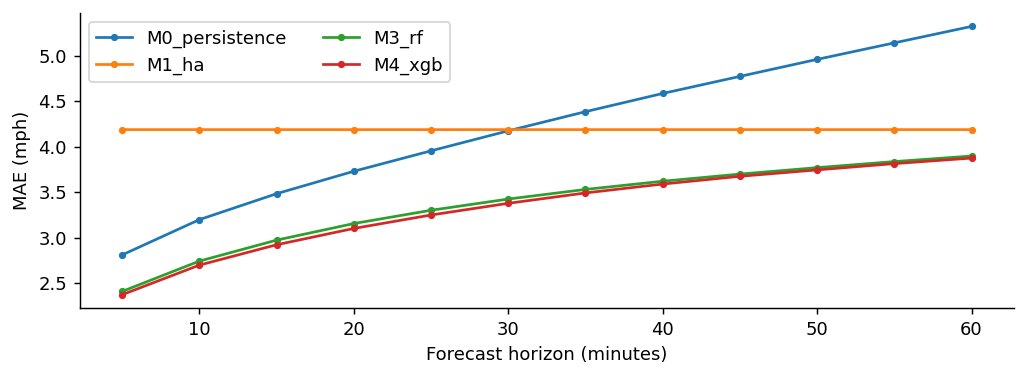
\includegraphics[width=\columnwidth]{mae_horizons_test.png}
\caption{Test MAE for all 12 horizons (5--60 minutes).}
\label{fig:horizon}
\end{figure}

The validation periods show the same ranking (Table~\ref{tab:val}). On val-2, Random Forest has a slightly lower 60-minute MAE than XGBoost, so the two learned models are close at long horizons.

\begin{table}[t]
\centering
\caption{Validation MAE (mph)}
\label{tab:val}
\begin{tabular}{l ccc ccc}
\toprule
& \multicolumn{3}{c}{Val-tune} & \multicolumn{3}{c}{Val-2} \\
\cmidrule(lr){2-4}\cmidrule(lr){5-7}
Model & 15 & 30 & 60 & 15 & 30 & 60 \\
\midrule
Persistence & 3.10 & 3.65 & 4.47 & 3.35 & 4.01 & 5.14 \\
Hist.\ average & 4.60 & 4.60 & 4.58 & 4.05 & 4.06 & 4.06 \\
Random Forest & 2.79 & 3.29 & 3.85 & 2.86 & 3.30 & \textbf{3.75} \\
XGBoost & \textbf{2.61} & \textbf{3.08} & \textbf{3.61} & \textbf{2.82} & \textbf{3.28} & 3.77 \\
\bottomrule
\end{tabular}
\end{table}

\subsection{Peak versus off-peak}
Table~\ref{tab:peak} and Fig.~\ref{fig:peak} split the test errors by time period. Errors during peak hours are roughly twice as large as off-peak for every model, because congestion starts and ends suddenly. At 60 minutes during peak hours Random Forest is clearly better than XGBoost (MAE 5.95 vs 6.31, RMSE 9.91 vs 11.56), while XGBoost has the lower MAE off-peak and at weekends. A single overall number would hide this.

\begin{table}[t]
\centering
\caption{Test MAE / RMSE (mph) by period, 60 minutes ahead}
\label{tab:peak}
\resizebox{\columnwidth}{!}{%
\begin{tabular}{lcccc}
\toprule
Model & Peak & Off-peak & Weekday & Weekend \\
\midrule
Persistence & 7.78 / 13.63 & 4.70 / 9.21 & 5.71 / 10.75 & 3.80 / 7.99 \\
Hist.\ avg. & 6.53 / 10.62 & 3.60 / 6.98 & 4.36 / 8.07 & 3.50 / 6.92 \\
RF & \textbf{5.95} / \textbf{9.91} & 3.38 / \textbf{6.42} & \textbf{4.04} / \textbf{7.43} & 3.33 / \textbf{6.51} \\
XGBoost & 6.31 / 11.56 & \textbf{3.26} / 6.81 & 4.07 / 8.25 & \textbf{3.10} / 6.89 \\
\bottomrule
\end{tabular}}
\end{table}

\begin{figure}[t]
\centering
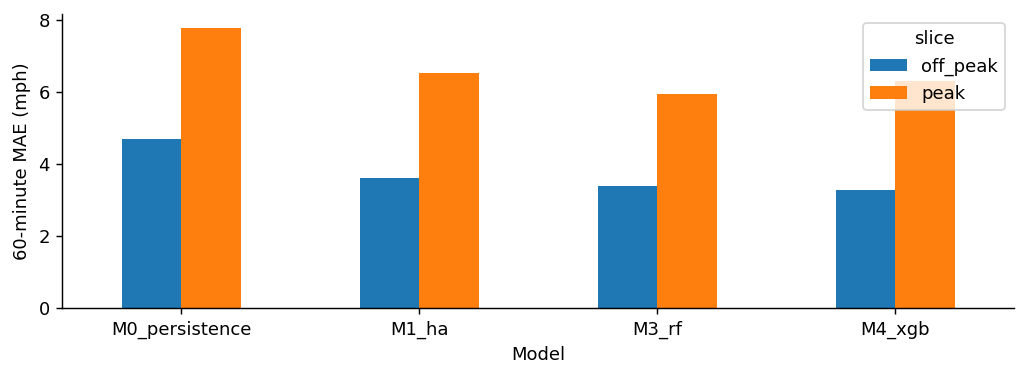
\includegraphics[width=\columnwidth]{peak_comparison_test.png}
\caption{60-minute test MAE in peak and off-peak hours.}
\label{fig:peak}
\end{figure}

\subsection{Per-sensor errors and error maps}
At 60 minutes, XGBoost has a lower MAE than persistence on 206 of the 207 sensors, with an average reduction of 1.45 mph per sensor. It beats Random Forest on 120 of 207 sensors, so neither model dominates everywhere. Fig.~\ref{fig:errormap} maps these per-sensor errors.

\begin{figure*}[t]
\centering
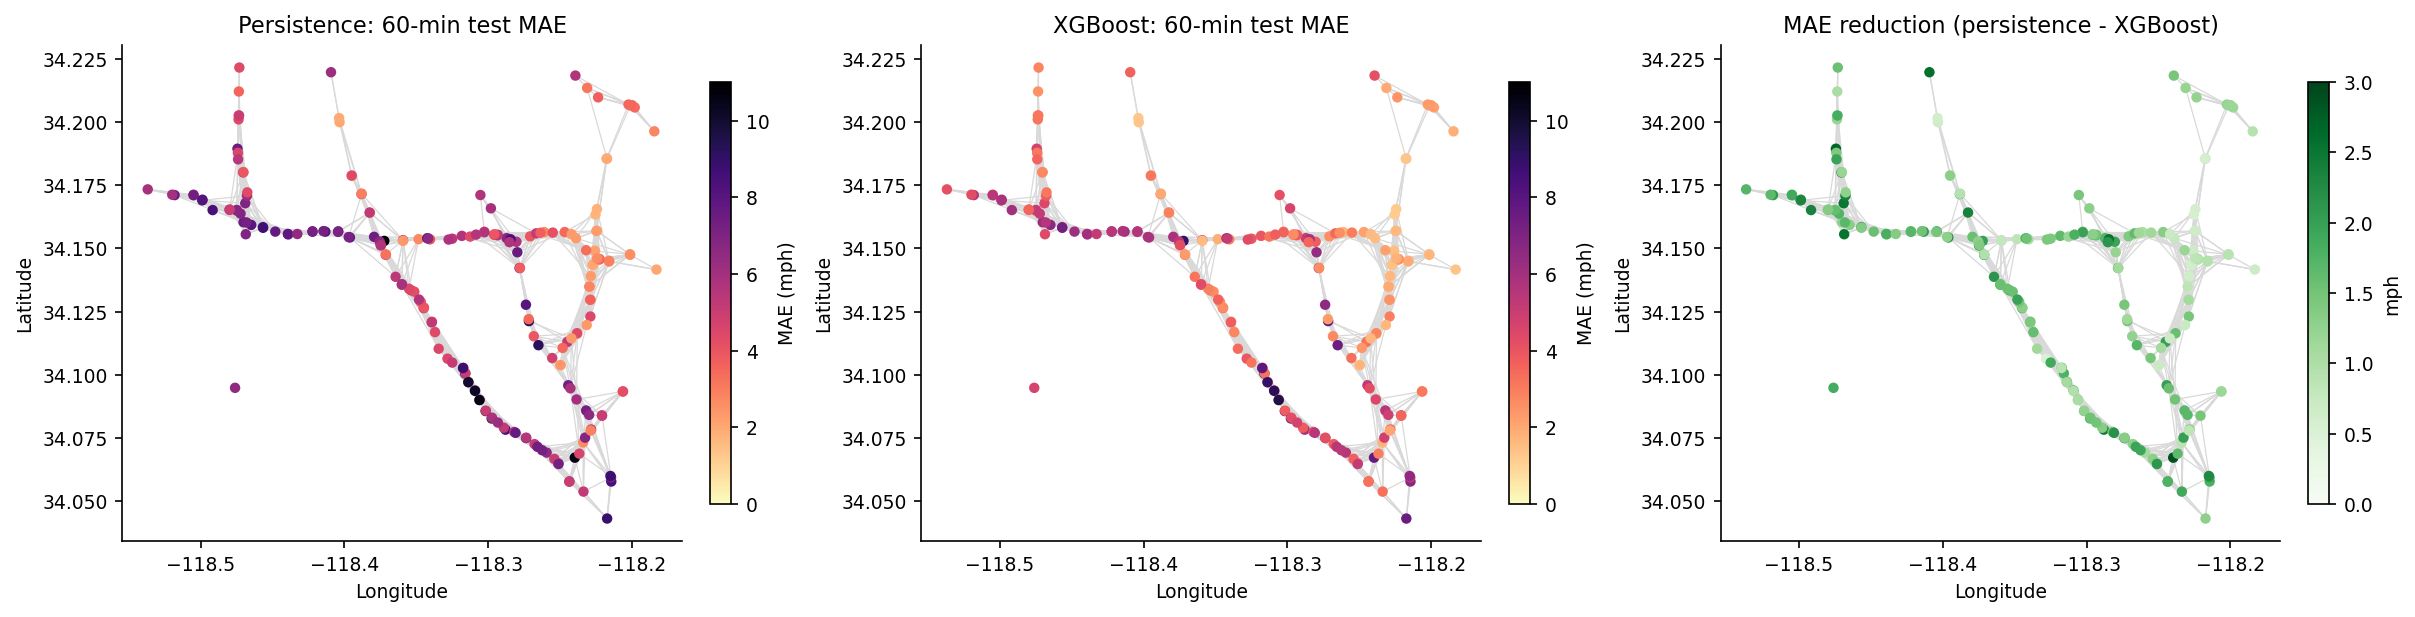
\includegraphics[width=\textwidth]{error_maps.png}
\caption{Forecast comparison maps: 60-minute test MAE of persistence (left) and XGBoost (centre) on the same colour scale, and the reduction achieved by XGBoost (right). The one sensor where XGBoost is slightly worse (by 0.10 mph) is shown at zero reduction.}
\label{fig:errormap}
\end{figure*}

\subsection{Example forecast}
Fig.~\ref{fig:example} shows 60-minute forecasts for one sensor on one test day. The sensor and day were fixed in advance by index, not chosen to make a model look good. Persistence is simply shifted by one hour. The learned models follow the morning jam much better but still miss its sharpest drops and react late to its end.

\begin{figure*}[t]
\centering
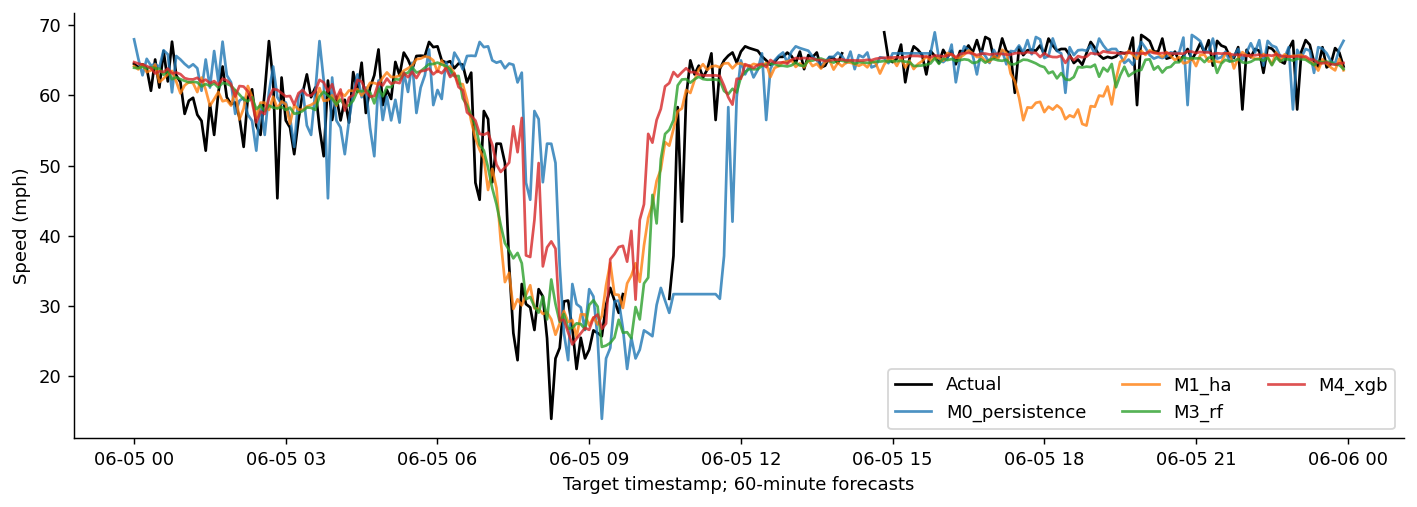
\includegraphics[width=0.85\textwidth]{forecast_example.png}
\caption{Actual speed and 60-minute-ahead forecasts for a fixed middle-index sensor on 5 June 2012.}
\label{fig:example}
\end{figure*}

\section{Discussion: The Gap Left by Independent Models}
\label{sec:gap}
The error maps in Fig.~\ref{fig:errormap} are not random: high-error sensors sit next to each other along specific corridors, especially the south-eastern diagonal highway, and the same corridors stay worst even for XGBoost. In the example of Fig.~\ref{fig:example}, the models react late to the start and end of the jam; a likely reason is that it builds up on nearby roads first. A per-sensor model only knows its own past. When congestion travels backwards from a downstream bottleneck, as the LWR theory predicts \cite{lighthill,richards}, the information that would warn our sensor is present in its neighbours' readings, which the model never receives.

This is the gap the brief asks us to identify. It gives a clear, testable hypothesis for Phase 2: a graph attention network \cite{gat} over the same road graph (Fig.~\ref{fig:congestion}), trained on the same splits, history window and masks, should reduce errors most at peak hours, at long horizons and on the high-error corridors. Our Phase 1 numbers are the baseline it must beat. Because the comparison protocol is already fixed, any improvement can be attributed to the use of neighbour information rather than to a different evaluation.

\section{Limitations}
\begin{itemize}
\item \textbf{Speed only.} METR-LA has no flow or occupancy, so the brief's flow and occupancy features cannot be built from this dataset.
\item \textbf{Test period seen earlier.} An earlier prototype's test results were inspected before this version, so we treat the test numbers as exploratory. No test result was used to choose any setting.
\item \textbf{Small tuning search.} Two candidates per model on six pilot sensors; better settings may exist.
\item \textbf{Training stride and label rules.} Training uses every second origin, and Random Forest drops rows with any missing future label, which removes some outage-related periods.
\item \textbf{Time zone.} The file stores clock times without a time zone, so peak hours refer to recorded clock time.
\item \textbf{MAPE.} MAPE is sensitive to low speeds and should be read together with MAE and RMSE.
\item \textbf{Negative forecasts.} 24 of 17,015,400 raw XGBoost test forecasts are slightly negative. They are kept as-is in the scores rather than clipped after seeing the results.
\item \textbf{One region and period.} Results come from four months of one city's highways.
\end{itemize}

\section{Reproducibility and Code Quality}
\label{sec:repro}
The project is a Python package (\texttt{src/trafficml}) with separate modules for data loading and graph building, masking and splits, features, models, evaluation and visualisation, plus command-line scripts:
\begin{itemize}
\item \texttt{scripts/check\_data.py}: verifies the dataset and adjacency;
\item \texttt{scripts/run\_all.py}: tunes, trains, evaluates and draws figures for a fresh run directory;
\item \texttt{scripts/predict.py}: forecasts 15/30/60 minutes for any sensor from saved models.
\end{itemize}
Dependencies are pinned in \texttt{requirements.txt} (Python 3.12). Every run writes a manifest with SHA-256 hashes of the data, configuration and source code, the selected parameters and the timings; the analysis, report and prediction scripts refuse to use a run if any of these have changed. The test suite (56 tests) checks causal features, purged splits, masks, metrics, model label rules, saved-model reloading and real-data shape and adjacency. A GitHub Actions workflow runs the tests, \texttt{ruff} lint and format checks on every push. Raw data, trained models and prediction arrays are kept out of Git.

\section{Team Contributions}
\label{sec:team}
The work was divided into five modules. Each member integrated and reviewed their module through a separate pull request to the team repository (Table~\ref{tab:team}).

\begin{table}[t]
\centering
\caption{Module responsibilities}
\label{tab:team}
\footnotesize
\begin{tabular}{>{\raggedright\arraybackslash}p{0.28\columnwidth}>{\raggedright\arraybackslash}p{0.5\columnwidth}l}
\toprule
Member & Module & PR \\
\midrule
Rudraksh Sharma & Dataset provenance, loading, sensor graph and adjacency checks & \#2 \\
Vridhi Chaudhary & Missing-data masking, chronological splits, feature engineering & \#3 \\
Anshuman Mehta & Exploratory data analysis and figures & \#4 \\
Bineet Keshari & Baselines, Random Forest and error analysis & \#5 \\
Kavya Katal & XGBoost, evaluation, reproducibility, report and integration & \#6 \\
\bottomrule
\end{tabular}
\end{table}

\textbf{Disclosure.} The integrated implementation builds on an earlier teammate prototype and was prepared with substantial AI assistance for coding, debugging, analysis and documentation. Module responsibility above describes who integrated and reviewed each part; each member is responsible for understanding and explaining the whole project in the individual viva.

\section{Conclusion and Future Work}
We built a leakage-safe, reproducible forecasting pipeline for 207 METR-LA sensors and showed that per-sensor tree ensembles clearly beat persistence and historical averages, reducing 60-minute MAE by about 27\%. XGBoost is best on MAE overall; Random Forest is best on RMSE and during peak hours at long horizons. Errors are largest at rush hour and cluster along corridors, which points to the missing ingredient: information from neighbouring roads.

\textbf{Phase 2 plan.}
\begin{enumerate}
\item Train a GAT or diffusion graph model in PyTorch Geometric on the verified adjacency matrix, with the same splits, 60-minute window and masks.
\item Compare it with the Phase 1 models by horizon, peak versus off-peak, and on the map; run ablations (no graph, fixed versus learned attention).
\item Try a justified hybrid, e.g.\ a graph model that corrects the XGBoost forecast using neighbour information.
\item Optionally extend to PeMS for flow and occupancy, and test a simple signal policy in simulation only (SUMO or CityFlow), never on real traffic.
\end{enumerate}

\begin{thebibliography}{10}
\bibitem{williams} B.~M. Williams and L.~A. Hoel, ``Modeling and forecasting vehicular traffic flow as a seasonal ARIMA process,'' \emph{J. Transp. Eng.}, vol.~129, no.~6, pp.~664--672, 2003.
\bibitem{castro} M.~Castro-Neto, Y.-S. Jeong, M.-K. Jeong, and L.~D. Han, ``Online-SVR for short-term traffic flow prediction under typical and atypical traffic conditions,'' \emph{Expert Syst. Appl.}, vol.~36, no.~3, pp.~6164--6173, 2009.
\bibitem{breiman} L.~Breiman, ``Random forests,'' \emph{Mach. Learn.}, vol.~45, pp.~5--32, 2001.
\bibitem{chen} T.~Chen and C.~Guestrin, ``XGBoost: A scalable tree boosting system,'' in \emph{Proc. KDD}, 2016, pp.~785--794.
\bibitem{hyndman} R.~J. Hyndman and A.~B. Koehler, ``Another look at measures of forecast accuracy,'' \emph{Int. J. Forecast.}, vol.~22, no.~4, pp.~679--688, 2006.
\bibitem{li} Y.~Li, R.~Yu, C.~Shahabi, and Y.~Liu, ``Diffusion convolutional recurrent neural network: Data-driven traffic forecasting,'' in \emph{Proc. ICLR}, 2018, arXiv:1707.01926.
\bibitem{gat} P.~Veli\v{c}kovi\'{c}, G.~Cucurull, A.~Casanova, A.~Romero, P.~Li\`{o}, and Y.~Bengio, ``Graph attention networks,'' in \emph{Proc. ICLR}, 2018, arXiv:1710.10903.
\bibitem{lighthill} M.~J. Lighthill and G.~B. Whitham, ``On kinematic waves II. A theory of traffic flow on long crowded roads,'' \emph{Proc. R. Soc. Lond. A}, vol.~229, no.~1178, pp.~317--345, 1955.
\bibitem{richards} P.~I. Richards, ``Shock waves on the highway,'' \emph{Oper. Res.}, vol.~4, no.~1, pp.~42--51, 1956.
\bibitem{cityflow} H.~Zhang, S.~Feng, C.~Liu, Y.~Ding, Y.~Zhu, Z.~Zhou, W.~Zhang, Y.~Yu, H.~Jin, and Z.~Li, ``CityFlow: A multi-agent reinforcement learning environment for large scale city traffic scenario,'' in \emph{Proc. WWW}, 2019, doi:10.1145/3308558.3314139.
\bibitem{sumo} P.~A. Lopez \emph{et al.}, ``Microscopic traffic simulation using SUMO,'' in \emph{Proc. IEEE ITSC}, 2018, pp.~2575--2582.
\end{thebibliography}

\end{document}
